\subsection{Motivation}

\begin{frame}{Motivation}
	\begin{mycolumns}[widths={50,50},animation=none]
		\begin{exampletight}{Modularization of Cross-Cutting Concerns}
			\centering
			\pic[width=1.0\linewidth]{aop-motivation-1} % todo: replace with picture from public domain
		\end{exampletight}
		\begin{example}{Feature Traceability}
			find feature 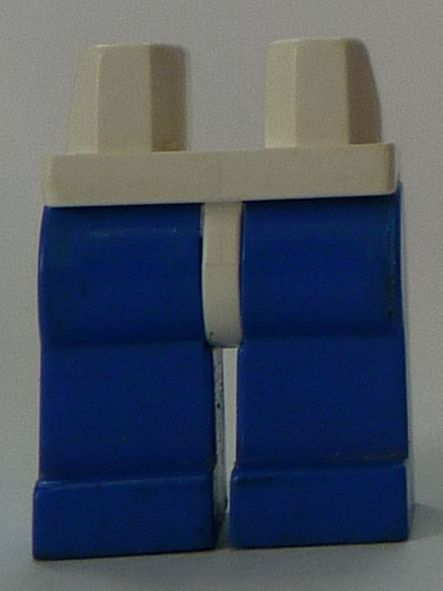
\includegraphics[width=.15\linewidth]{pants-blue} in product 
\includegraphics[width=.15\linewidth]{230}
		\end{example}
	\mynextcolumn
		\begin{exampletight}{Flexible Extension / Minimal Preplanning}
			\centering
			\pic[width=1.0\linewidth]{aop-motivation-2}
		\end{exampletight}
		
		~
		
		\begin{note}{}
			Achieving all this requires novel implementation techniques that overcome the limitations of classical object-oriented paradigms.
		\end{note}
	\end{mycolumns}
\end{frame}

\subsection{Feature Modules}

\begin{frame}{Background: Collaboration-Based Design} % TODO: is this original source ? \mytitlesource{Reenskaug et al.\ 1992}
	\begin{mycolumns}[widths={50,50},animation=none]
		\begin{definition}{Inspiration: Collaborations in the Real World}
			\begin{itemize}
				\item People collaborate to achieve a common goal.
				\item A collaboration typically comprises several persons playing different roles.
				\item Persons may play multiple roles by participating in different collaborations.
			\end{itemize}
		\end{definition}
		\begin{example}{Mentor-Student Collaboration}
			\begin{itemize}
				\item A person in the role of a mentor has responsibilities to instruct students on certain topics.
				\item A person in the role of a student has responsibilities to study the offered material.
			\end{itemize}
		\end{example}
	\mynextcolumn
		\pause
		\begin{definition}{Collaborations in Java \mysource{\fospl\mypages{131}}}
			\begin{itemize}
				\item A \emph{collaboration} is a set of interacting classes, each class playing a distinct role, to achieve a certain function or capability. 
				\item A \emph{role} defines the responsibilities a class takes in a collaboration.
			\end{itemize}
		\end{definition}
		\begin{note}{}
			\begin{itemize}
				\item Different classes play different roles within a collaboration.
				\item A class plays different roles in different collaborations.
				\item A role encapsulates the behavior/functionality of a class relevant to a collaboration.
			\end{itemize}
		\end{note}
	\end{mycolumns}
\end{frame}

\begin{frame}{Example: Collaborations, Classes and Roles}
	\begin{exampletight}{}
		\centering
		\pic[width=1.0\linewidth]{collaborations}
	\end{exampletight}
\end{frame}

\subsection{Feature Composition}

\begin{frame}{Feature Modules and Feature Module Composition}
	\begin{mycolumns}[widths={65,35},animation=none]
		\begin{definition}{Feature Modules}
			\begin{itemize}
				\item Each collaboration maps to a feature and is called a feature module (or layer).
				\item Feature modules may refine a base implementation by adding new elements or by modifying and extending existing ones.
			\end{itemize}
		\end{definition}
	\mynextcolumn
		\begin{definition}{Feature Module Composition}
			Selected feature modules may be superimposed by lining-up classes according to the roles they play.
		\end{definition}
	\end{mycolumns}
	\begin{exampletight}{}
		\centering
		\pic[width=0.95\linewidth]{feature-modules}
	\end{exampletight}
\end{frame}

\begin{frame}{Feature Modules and Feature Module Composition}
	\begin{note}{Open Questions}
		\begin{itemize}
			\item How to bundle classes to feature modules and specify their refinements?
			\item How to handle refinements during composition of feature modules?
		\end{itemize}
	\end{note}
	\begin{exampletight}{}
		\centering
		\pic[width=1.0\linewidth]{feature-modules}
	\end{exampletight}
\end{frame}

\subsection{FOP in Java}

\begin{frame}{Jak: A Java Extension for Feature-Oriented Programming \mytitlesource{Batory et al.\ 2004}}
	\begin{mycolumns}[widths={50,50},animation=none]
		\begin{definition}{Layers}
			\begin{itemize}
				\item The keyword layer denotes the feature a class belongs to.
				\item A layer is a set of files that define a feature of an application.
			\end{itemize}
		\end{definition}
		\begin{definition}{Class Refinement}
			A class refinement (keyword refines) can add new members to a class and extend existing methods. 
		\end{definition}
		\begin{definition}{Composer}
			\begin{itemize}
				\item AHEAD (Algebraic Hierarchical Equations for Application Design) + jampack/mixin
				\item Application constructed by composing layers
				\item Internally, the composer invokes a variety of tools to perform its task
			\end{itemize}
		\end{definition}
	\mynextcolumn
		\begin{exampletight}{Composer (High-Level View)}
			\centering
			\pic[width=1.0\linewidth]{AHEAD-composer}
		\end{exampletight}
		
		~
		
		\begin{exampletight}{Composer (Jak File Composition)}
			\centering
			\pic[width=1.0\linewidth]{AHEAD-jampack-mixin}
		\end{exampletight}
	\end{mycolumns}
\end{frame}

\begin{frame}[fragile]{Jak: Layers}
	\begin{mycolumns}[widths={60,40},animation=none]
		\begin{example}{}
			\begin{itemize}
				\item Layer (i.e., feature module) Base consists of the classes Graph, Node, and Edge 
				\item The three classes collaborate to provide the functionality to construct and display graph structures.
			\end{itemize}
		\end{example}
	\mynextcolumn
		\vspace{-1.5cm}\begin{flushright}\pic[width=3.8cm]{fop-horizontal}\end{flushright}
	\end{mycolumns}
	\begin{mycolumns}[columns=3,widths={43,27,30},animation=none]
\begin{codetight}{Graph.jak}
class Graph {
	private List nodes = new ArrayList();
	private List edges = new ArrayList();
	
	Edge add(Node n, Node m) {
		Edge e = new Edge(n, m);
		nodes.add(n); nodes.add(m); edges.add(e);
		return e;
	}
	void print() { ... }
}
\end{codetight}		
	\mynextcolumn
\begin{codetight}{Node.jak}
class Node {
	private int id = 0;

	void print() {
		System.out.print(id);
	}
}
~
~
~
~
~
\end{codetight}
	\mynextcolumn
\begin{codetight}{Edge.jak}
class Edge {
	private Node a, b;
	
	Edge(Node _a, Node _b) {
		a = _a; b = _b;
	}
	void print() {
		a.print(); b.print();
	}
}
~
~
\end{codetight}			
	\end{mycolumns}
\end{frame}

\begin{frame}[fragile]{Jak: Class Refinment – New Members}
	\vspace{-1.5cm}\begin{flushright}\pic[width=3.0cm]{fop-vertical}\end{flushright}
	\begin{mycolumns}[widths={50,50},animation=none]
		\begin{definition}{Mixin-Based Inheritance}
			Subclasses, called mixins, are abstract in the sense that they can be applied to \emph{different} concrete superclasses.
		\end{definition}
		\begin{definition}{Refinement Chain}
			A refinement chain is a linear inheritance chain where the bottom-most class of the chain is the only class that is meant to be instantiated.
		\end{definition}
		\begin{definition}{New Members}
			A stepwise refinement can add new members (i.e., fields and methods) to a class.
		\end{definition}
	\mynextcolumn
{\small
\begin{codetight}{Edge.jak}
class Edge {
	...
}
\end{codetight}
\begin{codetight}{Edge.jak}
refines class Edge {
	@private Node start;@
	...
}
\end{codetight}
\begin{codetight}{Edge.jak}
refines class Edge {
	@private Weight weight;@
	...
}
\end{codetight}
}
	\end{mycolumns}
\end{frame}

\begin{frame}[fragile]{Jak: Class Refinement – Method Extensions}
	\vspace{-1.5cm}\begin{flushright}\pic[width=2.8cm]{fop-vertical}\end{flushright}
	\begin{mycolumns}[widths={50,50},animation=none]
		\begin{definition}{Mixin-Based Inheritance}
			Subclasses, called mixins, are abstract in the sense that they can be applied to \emph{different} concrete superclasses.
		\end{definition}
		\begin{definition}{Refinement Chain}
			A refinement chain is a linear inheritance chain where the bottom-most class of the chain is the only class that is meant to be instantiated.
		\end{definition}
		\begin{definition}{Method Extension}
			A method extension is implemented by method overriding and calling the overridden method via the keyword Super.
		\end{definition}
	\mynextcolumn
{
\begin{codetight}[basicstyle=\tiny]{Edge.jak}
class Edge {
	void print() {
		System.out.print("Edge between " + a + " and " + b);
	}
}
\end{codetight}
\begin{codetight}[basicstyle=\tiny]{Edge.jak}
refines class Edge {
	...
	void print() {
		@Super().print();@
		@System.out.print(" directed from " + start);@
	}
}
\end{codetight}
\begin{codetight}[basicstyle=\tiny]{Edge.jak}
refines class Edge {
	...
	void print() {
		@Super().print();@
		@System.out.print(" weighted with " + weight);@
	}
}
\end{codetight}
}
	\end{mycolumns}
\end{frame}

\begin{frame}[fragile]{AHEAD: Composition Using Jampack}
	\begin{mycolumns}[widths={35,65},animation=none]
		\begin{definition}{Jampack}
			\begin{itemize}
				\item Jampack superimposes the refinement chain into a single class.
				\item Super calls are integrated by method inlining (cf.\ optimization in compiler construction).
			\end{itemize}
		\end{definition}
	\mynextcolumn
\begin{codetight}{Composition Result}
class Edge {
	private Node start;
	private Weight weight;
	void print() {
		System.out.print("Edge between " + a + " and " + b);
		System.out.print(" directed from " + start);
		System.out.print(" weighted with " + weight);
	}
}
\end{codetight}
	\end{mycolumns}
\end{frame}

\begin{frame}[fragile]{AHEAD: Composition Using Mixin}
	\begin{mycolumns}[widths={50,50},animation=none]
		\begin{definition}{Mixin}
			\begin{itemize}
				\item Mixin retains layer relationships as an inheritance chain.  
				\item Produces a single file that contains a (linear) inheritance hierarchy where only the bottom-most class is ``public''.
				\item Super calls are integrated by method inlining (cf.\ optimization in compiler construction).
			\end{itemize}
		\end{definition}
	\mynextcolumn
{\small
\begin{codetight}{Composition Result}
class Edge$$Base {
	void print() { ... }
}
class Edge$$Directed extends Edge$$Base {
	private Node start;
	void print() {
		super.print();
		System.out.print(" directed from " + start);
	}
}
class Edge extends Edge$$Directed {
	private Weight weight;
	void print() {
		super.print();
		System.out.print(" weighted with " + weight);
	}
}
\end{codetight}
}
	\end{mycolumns}
\end{frame}

\begin{frame}{Jampack vs. Mixin}
	\begin{mycolumns}[widths={50,50},animation=none]
		\begin{note}{Jampack}
			\begin{itemize}
				\item Assignment of generated code to roles disappears after generation 
				\item Local variables can be accessed from within refined methods
			\end{itemize}
		\end{note}
	\mynextcolumn
		\begin{note}{Mixin}
			\begin{itemize}
				\item Code overhead and method call indirections negatively impact runtime performance
				\item Feature modularity preserved even after composition
			\end{itemize}
		\end{note}
	\end{mycolumns}
\end{frame}

\begin{frame}{Jampack and Mixin in Practice }
	\begin{mycolumns}[widths={50,50},animation=none]
		\begin{note}{Recommended Usage}
			\begin{itemize}
				\item Use Mixin during development and iterative refinement (debugging)
				\item Use Jampack when a production version of a class is to be produced (performance)
			\end{itemize}
		\end{note}
		\begin{definition}{Unmixin}
			Automatically propagates changes from the composed .jak file back to its original layer files
		\end{definition}
	\mynextcolumn
		\begin{note}{Unmixin and Debugging}
			\begin{itemize}
				\item Make changes to a mixin-composed .jak file during debugging 
				\item Then automatically back-propagate changes to the layer files
			\end{itemize}
		\end{note}
		\begin{exampletight}{}
			\centering
			\pic[width=1.0\linewidth]{AHEAD-unmixin}
		\end{exampletight}
	\end{mycolumns}
\end{frame}

\begin{frame}[fragile]{Composition: Order Matters!}
	\begin{note}{}
		Class refinements themselves are (largely) independent of the order in which they are eventually composed.
	\end{note}
	\pause
	\begin{mycolumns}[widths={50,50},animation=none]
{
\begin{codetight}[basicstyle=\tiny]{(a) Edge.jak}
class Edge {
	void print() {
		System.out.print("Edge between " + a + " and " + b);
	}
}
\end{codetight}
\begin{codetight}[basicstyle=\tiny]{(b) Edge.jak}
refines class Edge { ...
	void print() {
		Super().print();
		System.out.print(" directed from " + start);
	}
}
\end{codetight}
\begin{codetight}[basicstyle=\tiny]{(c) Edge.jak}
refines class Edge { ...
	void print() {
		Super().print();
		System.out.print(" weighted with " + weight);
	}
}
\end{codetight}
}
	\mynextcolumn
		\pause
		\begin{note}{}
			However, the order in which features are applied is important 
			(e.g., earlier features in the sequence may add elements that are refined by later features). 
		\end{note}
\begin{codetight}{Composition Order (a),(b),(c)}
class Edge {
	private Node start;
	private Weight weight;
	void print() {
		System.out.print("Edge between " + a + " and " + b);
		System.out.print(" directed from " + start);
		System.out.print(" weighted with " + weight);
	}
}
\end{codetight}
	\end{mycolumns}
\end{frame}

\begin{frame}[fragile]{Composition: Order Matters!}
	\begin{note}{}
		Class refinements themselves are (largely) independent of the order in which they are eventually composed.
	\end{note}
	\begin{mycolumns}[widths={50,50},animation=none]
{
\begin{codetight}[basicstyle=\tiny]{(a) Edge.jak}
class Edge {
	void print() {
		System.out.print("Edge between " + a + " and " + b);
	}
}
\end{codetight}
\begin{codetight}[basicstyle=\tiny]{(b) Edge.jak}
refines class Edge { ...
	void print() {
		Super().print();
		System.out.print(" directed from " + start);
	}
}
\end{codetight}
\begin{codetight}[basicstyle=\tiny]{(c) Edge.jak}
refines class Edge { ...
	void print() {
		Super().print();
		System.out.print(" weighted with " + weight);
	}
}
\end{codetight}
}
	\mynextcolumn
		\begin{note}{}
			However, the order in which features are applied is important 
			(e.g., earlier features in the sequence may add elements that are refined by later features). 
		\end{note}
\begin{codetight}{Composition Order (a),(c),(b)}
class Edge {
	private Node start;
	private Weight weight;
	void print() {
		System.out.print("Edge between " + a + " and " + b);
		System.out.print(" weighted with " + weight);
		System.out.print(" directed from " + start);
	}
}
\end{codetight}
	\end{mycolumns}
\end{frame}

\begin{frame}{Composition: Order Matters!}
	\begin{mycolumns}[widths={50,50},animation=none]
		\begin{note}{}
			The order in which compositions are to be applied is an input parameter of the composer tool.
		\end{note}
		\pause
		\begin{note}{Composition order in FeatureIDE}
			\begin{itemize}
				\item In FeatureIDE, a total order can be defined based on the feature model
				\item Default: Depth-first traversal of the feature model
			\end{itemize}
		\end{note}
	\mynextcolumn
		\begin{exampletight}{}
			\centering\featureDiagramGraphs
			\featureDiagramLegend
		\end{exampletight}
	\end{mycolumns}
\end{frame}

\begin{frame}{Big Picture: Product-Line Implementation and Product Generation}
	\begin{center}
		\only<1| handout:0>{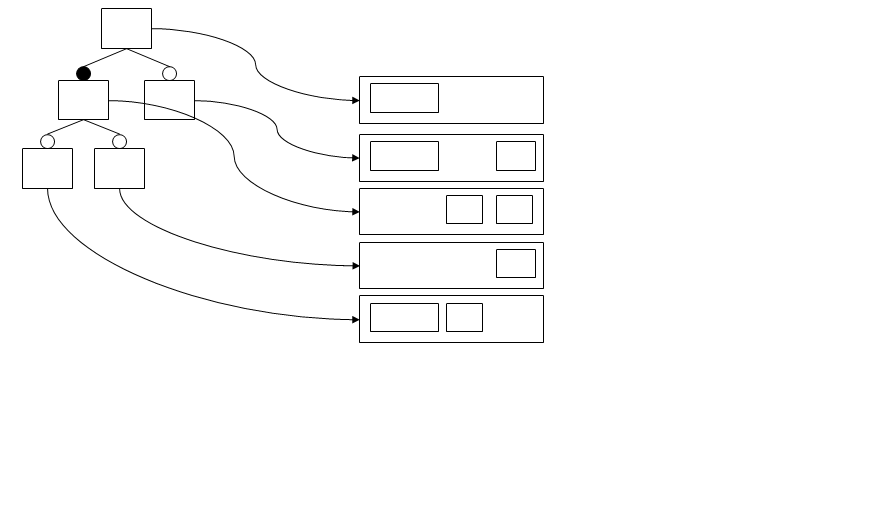
\includegraphics[height=0.8\textheight]{feature_komposition1}}
		\only<2| handout:0>{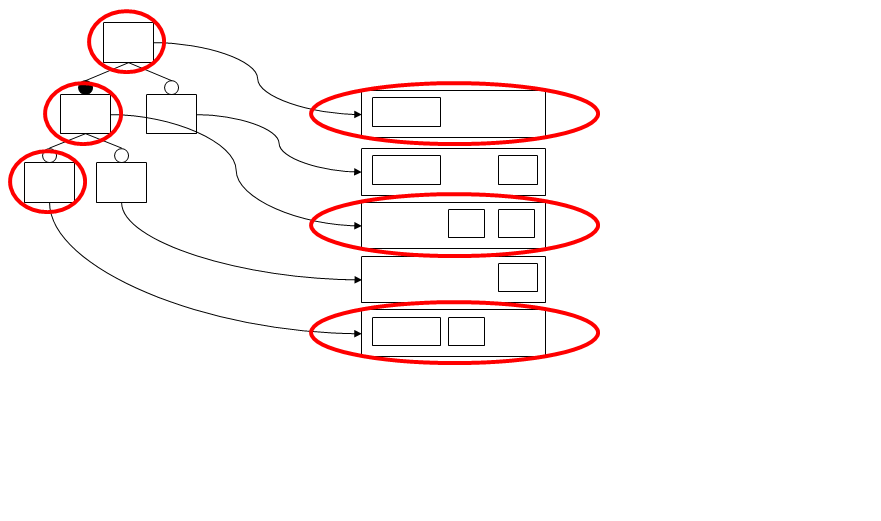
\includegraphics[height=0.8\textheight]{feature_komposition2}}
		\only<3| handout:0>{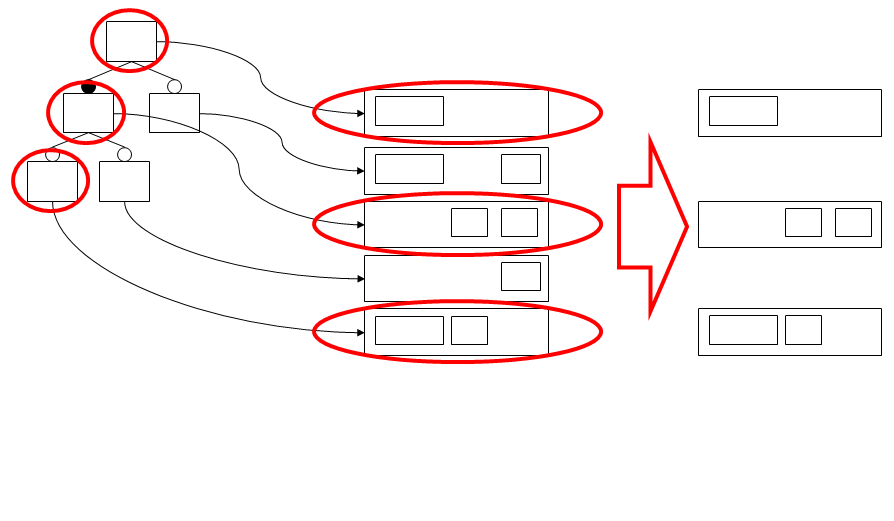
\includegraphics[height=0.8\textheight]{feature_komposition3}}
		\only<4>{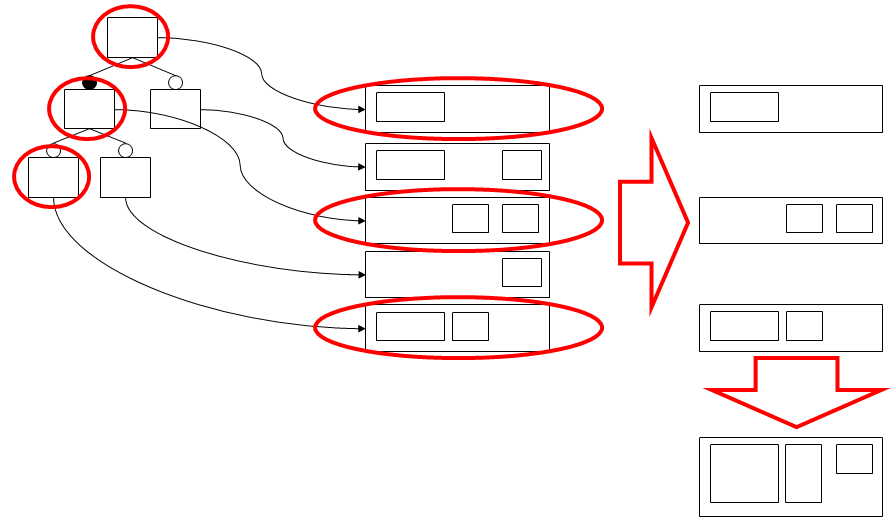
\includegraphics[height=0.8\textheight]{feature_komposition4}}
	\end{center}
\end{frame}

\begin{frame}{Practical Organization of Feature Modules}
	\begin{mycolumns}[widths={70,30},animation=none]
		\begin{exampletight}{}
			\centering
			\pic[width=1.0\linewidth]{fop-directories-fide}
		\end{exampletight}
	\mynextcolumn
		\begin{note}{}
			\begin{itemize}
				\item In most FOP tools, feature modules are represented by (nested) file-system directories
				\item Classes and their refinements are stored in files inside the corresponding containment hierarchies
			\end{itemize}
		\end{note}
	\end{mycolumns}
\end{frame}

\subsection{Principle of Uniformity}

\begin{frame}{Beyond Jak: Uniformity}
	\begin{mycolumns}[widths={35,65},animation=none]
		\begin{note}{Motivation}
			\begin{itemize}
				\item Software does not only consist of Java source code, but also other programming languages, build scripts, documentation, models, etc.
				\item All software artifacts must be refined 
				\item Integration of different artifacts in collaborations
			\end{itemize}
		\end{note}
	\mynextcolumn
		\begin{definition}{Idea}
			\begin{itemize}
				\item Each feature is represented by a containment hierarchy: 
				\begin{itemize}
					\item Directory structure organizes the feature's artifacts.
					\item At the file level, there may be heterogeneous artifacts.
				\end{itemize}
				\item Composing features means composing containment hierarchies and, to this end, composing corresponding artifacts recursively by name and type
				\item For each artifact type, a different implementation of the composition operator ``$\bullet$'' has to be provided in AHEAD (just like the Jak-composition tool)
			\end{itemize}
		\end{definition}
	\end{mycolumns}
\end{frame}

\begin{frame}{Beyond Jak: Uniformity}
	\begin{exampletight}{}
		\centering
		\pic[width=1.0\linewidth]{composition_dir}
	\end{exampletight}
\end{frame}

\begin{frame}{FeatureHouse: A Model and Framework for FOP}
	\begin{mycolumns}[widths={50,50},animation=none]
		\begin{definition}{Goal}
			\emph{Language-independent model and tool chain} to enhance given languages rapidly with support for feature-oriented programming
		\end{definition}
		\begin{definition}{Assumption}
			\begin{itemize}
				\item A feature may be represented as tree, known as \emph{Feature Structure Tree (FST)}
				\item Example; Java: Packages, Classes, Methods and Fields 
			\end{itemize}
		\end{definition}
	\mynextcolumn
		\begin{definition}{Idea}
			\begin{itemize}
				\item Composition = Superimposition of FSTs (i.e., recursively superimpose nodes of FST, starting with the root node)
				\item Inner nodes: Can be safely superimposed if they are identical (superimposed parents and same name), or added if non-identical
				\item Leaf nodes: Type-specific resolution of conflicts
			\end{itemize}
		\end{definition}
	\end{mycolumns}
\end{frame}

\begin{frame}{FeatureHouse: Overview}
	\begin{exampletight}{}
		\centering
		\pic[width=0.85\linewidth]{featurehouse}
	\end{exampletight}
\end{frame}

\begin{frame}{FeatureHouse: Composition}
	\begin{exampletight}{}
		\centering
		\pic[width=0.77\linewidth]{featurehouse_composition}
	\end{exampletight}
\end{frame}

\begin{frame}[fragile]{Example: Java Support in FeatureHouse}
	\begin{mycolumns}[widths={60,40},animation=none]
{\small
\begin{codetight}{}
class Edge {
	private Node a, b;
	void print() {
		System.out.print("Edge between " + a + " and " + b);
	}
}
\end{codetight}
\begin{codetight}{}
class Edge {
	private Node start;
	void print() {
		original();
		System.out.print(" directed from " + start);
	}
}
\end{codetight}
\begin{codetight}{}
class Edge {
	private Weight weight;
	void print() {
		original();
		System.out.print(" weighted with " + weight);
	}
}
\end{codetight}
}
	\mynextcolumn
		\begin{note}{Differences compared to Jak}
			\begin{itemize}
				\item No explicit keyword refines 
				\item Calling the method from previous refinement using keyword original
			\end{itemize}
		\end{note}
	\end{mycolumns}
\end{frame}

\subsection{Discussion}

\begin{frame}{Discussion}
	\begin{mycolumns}[widths={50,50},animation=none]
		\begin{note}{Advantages}
			\begin{itemize}
				\item Easy to use language-based mechanism, requires only minimal language extensions.
				\item Conceptually uniformly applicable to code and noncode artifacts.
				\item Separation of (possibly crosscutting) feature code into distinct feature modules.
				\item Little preplanning required due to mixin-based extension mechanism.
				\item Direct feature traceability from a feature to its implementation in a feature module.
			\end{itemize}
		\end{note}
	\mynextcolumn
		\begin{note}{Disadvantages}
			\begin{itemize}
				\item Requires adoption of a language extension and composition tools.
				\item Tools need to be constructed for every language (although with the help of a framework).
				\item Only academic tools so far, little experience in practice.
				\item Granularity restricted to method-level (or other named structural entities).
			\end{itemize}
		\end{note}
	\end{mycolumns}
\end{frame}

% TODO mention deltas?
% see spl07b.tex in old Latex slides (slides created by Thomas Thuem)
